% $Id: xmlreport.tex 12283 2010-09-23 10:34:38Z alexandra $
% Local Variables:
% ispell-check-comments: nil
% Local IspellDict: american
% End:
% --------------------------------------------------------
% User documentation
% copyright by BREDEX GmbH 2005
% --------------------------------------------------------
% this command can be inserted multiple times
%\gdhelpid{}
% 
%\begin{gddescription}
%\end{gddescription}
%
%\begin{gdlist}
% use the \item command for single steps
%\end{gdlist}
% change <PATH> to the same directory, file is located in
% change <FILE> to the same filename you are editing
%\bxinput{<PATH>/Links/<FILE>}
%
% other usefull commands are
%   \bxtipp{}        to create a hint
%   \bxwarn{}        to describe a warning
\index{XML and HTML Result Reports}
\index{Results!XML and HTML Reports}
You can create XML and HTML reports for your tests in one of two ways:

\begin{enumerate}
\item In the \gdtestsummaryview{} \bxpref{TestSummaryExport}.
\item You can specify that XML and HTML reports should be created when a test runs in the preferences  \bxpref{testresprefs}.
\begin{itemize}
\item We recommend using the option to export test results from the \gdtestsummaryview{}, as this does not involve defining any external files for your test environment. 
\end{itemize}
\end{enumerate}

%% \begin{figure}
%% 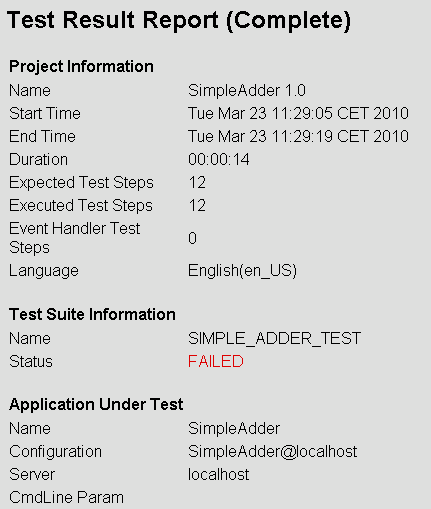
\includegraphics{Tasks/Testexecution/PS/htmlpart1}
%% \caption{HTML Report Part 1}
%% \label{htmlreport1}
%% \end{figure}
%% \begin{figure}
%% 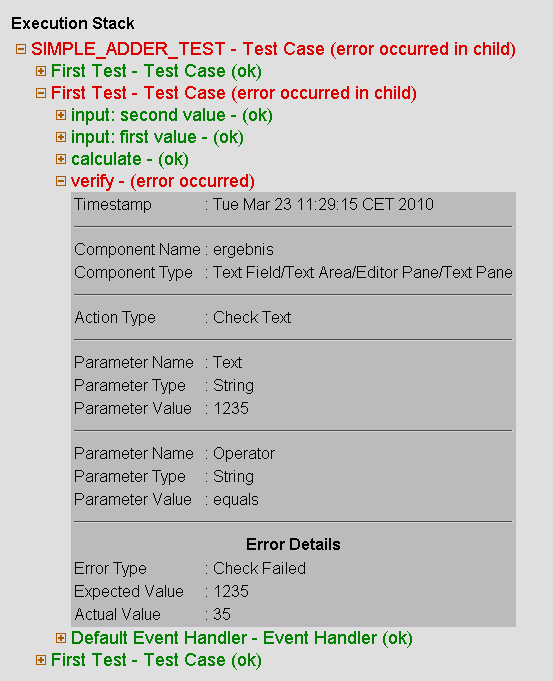
\includegraphics{Tasks/Testexecution/PS/htmlpart2}
%% \caption{HTML Report Part 2}
%% \label{htmlreport2}
%% \end{figure}

